\documentclass{beamer}\usepackage[]{graphicx}\usepackage[]{color}
%% maxwidth is the original width if it is less than linewidth
%% otherwise use linewidth (to make sure the graphics do not exceed the margin)
\makeatletter
\def\maxwidth{ %
  \ifdim\Gin@nat@width>\linewidth
    \linewidth
  \else
    \Gin@nat@width
  \fi
}
\makeatother

\definecolor{fgcolor}{rgb}{0.345, 0.345, 0.345}
\newcommand{\hlnum}[1]{\textcolor[rgb]{0.686,0.059,0.569}{#1}}%
\newcommand{\hlstr}[1]{\textcolor[rgb]{0.192,0.494,0.8}{#1}}%
\newcommand{\hlcom}[1]{\textcolor[rgb]{0.678,0.584,0.686}{\textit{#1}}}%
\newcommand{\hlopt}[1]{\textcolor[rgb]{0,0,0}{#1}}%
\newcommand{\hlstd}[1]{\textcolor[rgb]{0.345,0.345,0.345}{#1}}%
\newcommand{\hlkwa}[1]{\textcolor[rgb]{0.161,0.373,0.58}{\textbf{#1}}}%
\newcommand{\hlkwb}[1]{\textcolor[rgb]{0.69,0.353,0.396}{#1}}%
\newcommand{\hlkwc}[1]{\textcolor[rgb]{0.333,0.667,0.333}{#1}}%
\newcommand{\hlkwd}[1]{\textcolor[rgb]{0.737,0.353,0.396}{\textbf{#1}}}%

\usepackage{framed}
\makeatletter
\newenvironment{kframe}{%
 \def\at@end@of@kframe{}%
 \ifinner\ifhmode%
  \def\at@end@of@kframe{\end{minipage}}%
  \begin{minipage}{\columnwidth}%
 \fi\fi%
 \def\FrameCommand##1{\hskip\@totalleftmargin \hskip-\fboxsep
 \colorbox{shadecolor}{##1}\hskip-\fboxsep
     % There is no \\@totalrightmargin, so:
     \hskip-\linewidth \hskip-\@totalleftmargin \hskip\columnwidth}%
 \MakeFramed {\advance\hsize-\width
   \@totalleftmargin\z@ \linewidth\hsize
   \@setminipage}}%
 {\par\unskip\endMakeFramed%
 \at@end@of@kframe}
\makeatother

\definecolor{shadecolor}{rgb}{.97, .97, .97}
\definecolor{messagecolor}{rgb}{0, 0, 0}
\definecolor{warningcolor}{rgb}{1, 0, 1}
\definecolor{errorcolor}{rgb}{1, 0, 0}
\newenvironment{knitrout}{}{} % an empty environment to be redefined in TeX

\usepackage{alltt} 

\usepackage{graphics}
\usepackage[T1]{fontenc}
\setbeamercovered{transparent}
\renewcommand{\ni}{\noindent}
% \SweaveOpts{cache=TRUE, background="white"}

%load packages that will be invisible on slides



\title[ 1-Intro]{Day 1 - Intro to R}
\subtitle{Sneak Peek!}
\author[ K. Maurer, S. VanderPlas, E. Hare]{Karsten Maurer, Eric Hare, and Susan VanderPlas}
\date{February 12, 2014}
\institute[ISU]{Iowa State University}
\IfFileExists{upquote.sty}{\usepackage{upquote}}{}

\begin{document}

\begin{frame}
    \maketitle
\end{frame}

%-----------------------------------------------------------------------------

\begin{frame}
    \frametitle{Motivating Example}
    \begin{itemize}
        \item Kick off the workshop by exploring a real data set using R!
        \item Goal: get the flavor of using R for data management and exploration
        \item Don't worry about understanding all the coding right away
        \item We will go back and explain how it all works in detail
    \end{itemize}    
\end{frame}

%-----------------------------------------------------------------------------

\begin{frame}
    \frametitle{Tips Data Set}
    \begin{itemize}
        \item Tips data set recorded by a server in a restaurant over a span of about 10 weeks
        \item Server recorded several variables about groups they served:
        \begin{itemize} 
          \item Amount they were tipped
          \item Cost of the total bill
          \item Several characteristics about the groups being served
        \end{itemize}
        \item Primary Question: How do these variable influence the amount being tipped?
        \item Follow along using RWorkshop1Tips.R
    \end{itemize}    
\end{frame}

%-----------------------------------------------------------------------------

\begin{frame}[fragile]
    \frametitle{First look at data in R}
    
    Lets use R to look at the top few rows of the tips data set 
    
    \small
\begin{knitrout}\footnotesize
\definecolor{shadecolor}{rgb}{1, 1, 1}\color{fgcolor}\begin{kframe}
\begin{alltt}
\hlcom{# head() will pull the first few rows}
\hlkwd{head}\hlstd{(tips)}
\end{alltt}
\begin{verbatim}
##   total_bill  tip    sex smoker day   time size
## 1      16.99 1.01 Female     No Sun Dinner    2
## 2      10.34 1.66   Male     No Sun Dinner    3
## 3      21.01 3.50   Male     No Sun Dinner    3
## 4      23.68 3.31   Male     No Sun Dinner    2
## 5      24.59 3.61 Female     No Sun Dinner    4
## 6      25.29 4.71   Male     No Sun Dinner    4
\end{verbatim}
\end{kframe}
\end{knitrout}

    \normalsize
\end{frame}

%-----------------------------------------------------------------------------

\begin{frame}[fragile]
    \frametitle{Tips data attributes}
    
How big is this data set and what types of variables are in each column?

    \small
\begin{knitrout}\footnotesize
\definecolor{shadecolor}{rgb}{1, 1, 1}\color{fgcolor}\begin{kframe}
\begin{alltt}
\hlcom{# look at the structure of the tips data set}
\hlkwd{str}\hlstd{(tips)}
\end{alltt}
\begin{verbatim}
## 'data.frame':	244 obs. of  7 variables:
##  $ total_bill: num  17 10.3 21 23.7 24.6 ...
##  $ tip       : num  1.01 1.66 3.5 3.31 3.61 4.71 2 3.12 1.96 3.23 ...
##  $ sex       : Factor w/ 2 levels "Female","Male": 1 2 2 2 1 2 2 2 2 2 ...
##  $ smoker    : Factor w/ 2 levels "No","Yes": 1 1 1 1 1 1 1 1 1 1 ...
##  $ day       : Factor w/ 4 levels "Fri","Sat","Sun",..: 3 3 3 3 3 3 3 3 3 3 ...
##  $ time      : Factor w/ 2 levels "Dinner","Lunch": 1 1 1 1 1 1 1 1 1 1 ...
##  $ size      : int  2 3 3 2 4 4 2 4 2 2 ...
\end{verbatim}
\end{kframe}
\end{knitrout}

    \normalsize
\end{frame}

%-----------------------------------------------------------------------------

\begin{frame}[fragile]
    \frametitle{Tips Variables}

Let's get a summary of the values for each variable in tips

    \small
\begin{knitrout}\footnotesize
\definecolor{shadecolor}{rgb}{1, 1, 1}\color{fgcolor}\begin{kframe}
\begin{alltt}
\hlkwd{summary}\hlstd{(tips)}
\end{alltt}
\begin{verbatim}
##    total_bill         tip            sex      smoker      day    
##  Min.   : 3.07   Min.   : 1.00   Female: 87   No :151   Fri :19  
##  1st Qu.:13.35   1st Qu.: 2.00   Male  :157   Yes: 93   Sat :87  
##  Median :17.80   Median : 2.90                          Sun :76  
##  Mean   :19.79   Mean   : 3.00                          Thur:62  
##  3rd Qu.:24.13   3rd Qu.: 3.56                                   
##  Max.   :50.81   Max.   :10.00                                   
##      time          size     
##  Dinner:176   Min.   :1.00  
##  Lunch : 68   1st Qu.:2.00  
##               Median :2.00  
##               Mean   :2.57  
##               3rd Qu.:3.00  
##               Max.   :6.00
\end{verbatim}
\end{kframe}
\end{knitrout}

    \normalsize
\end{frame}

%-----------------------------------------------------------------------------


\begin{frame}[fragile]
    \frametitle{Scatterplots}

Lets look at the relationship between total bill and tip value

\small
\begin{knitrout}\footnotesize
\definecolor{shadecolor}{rgb}{1, 1, 1}\color{fgcolor}\begin{kframe}
\begin{alltt}
\hlkwd{qplot}\hlstd{(tip, total_bill,} \hlkwc{geom} \hlstd{=} \hlstr{"point"}\hlstd{,} \hlkwc{data} \hlstd{= tips)}
\end{alltt}
\end{kframe}
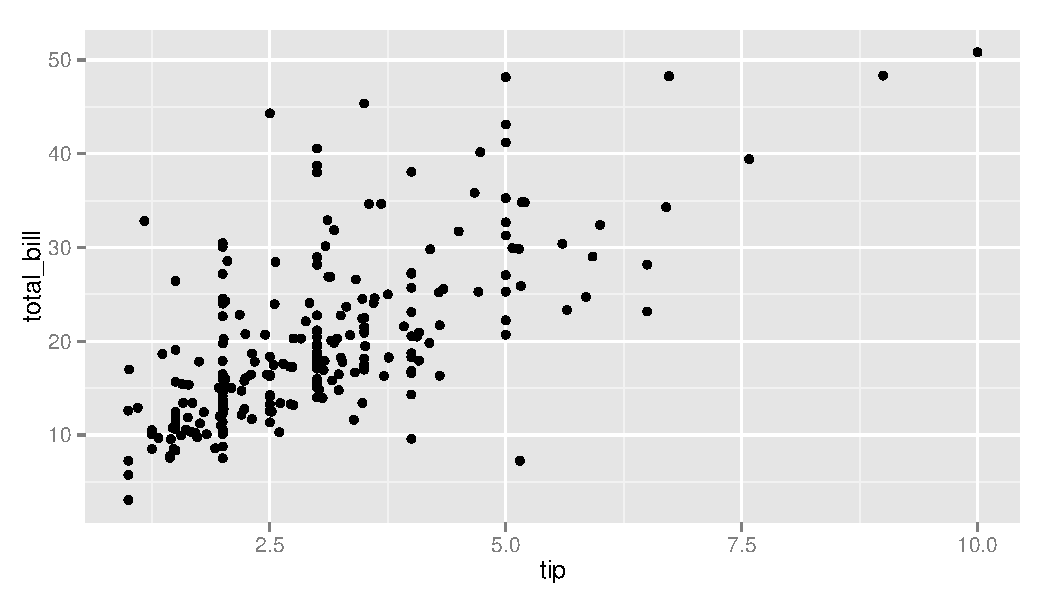
\includegraphics[width=\textwidth]{figure/kMEtipsscatter} 

\end{knitrout}

    \normalsize
\end{frame}

%-----------------------------------------------------------------------------

\begin{frame}[fragile]
    \frametitle{Scatterplots}

Color the points by lunch and dinner groups

\small
\begin{knitrout}\footnotesize
\definecolor{shadecolor}{rgb}{1, 1, 1}\color{fgcolor}\begin{kframe}
\begin{alltt}
\hlkwd{qplot}\hlstd{(tip, total_bill,} \hlkwc{geom} \hlstd{=} \hlstr{"point"}\hlstd{,} \hlkwc{data} \hlstd{= tips,} \hlkwc{colour} \hlstd{= time)}
\end{alltt}
\end{kframe}
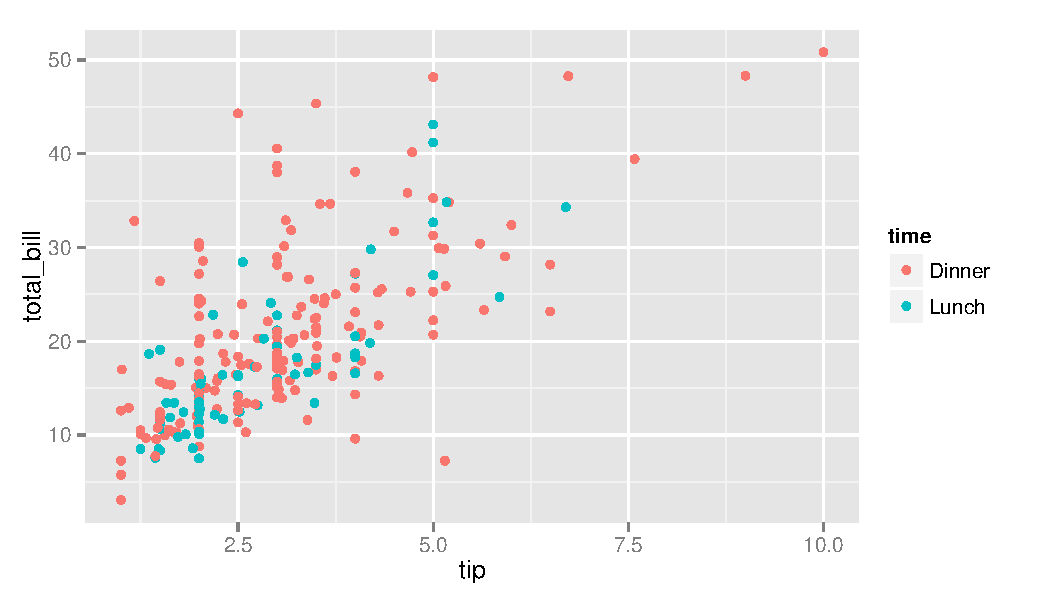
\includegraphics[width=\textwidth]{figure/kMEtipsscattercolor} 

\end{knitrout}

    \normalsize
\end{frame}

%-----------------------------------------------------------------------------

\begin{frame}[fragile]
    \frametitle{Scatterplots}

Add linear regression line to the plot

\small
\begin{knitrout}\footnotesize
\definecolor{shadecolor}{rgb}{1, 1, 1}\color{fgcolor}\begin{kframe}
\begin{alltt}
\hlkwd{qplot}\hlstd{(tip, total_bill,} \hlkwc{geom} \hlstd{=} \hlstr{"point"}\hlstd{,} \hlkwc{data} \hlstd{= tips)} \hlopt{+} \hlkwd{geom_smooth}\hlstd{(}\hlkwc{method} \hlstd{=} \hlstr{"lm"}\hlstd{)}
\end{alltt}
\end{kframe}
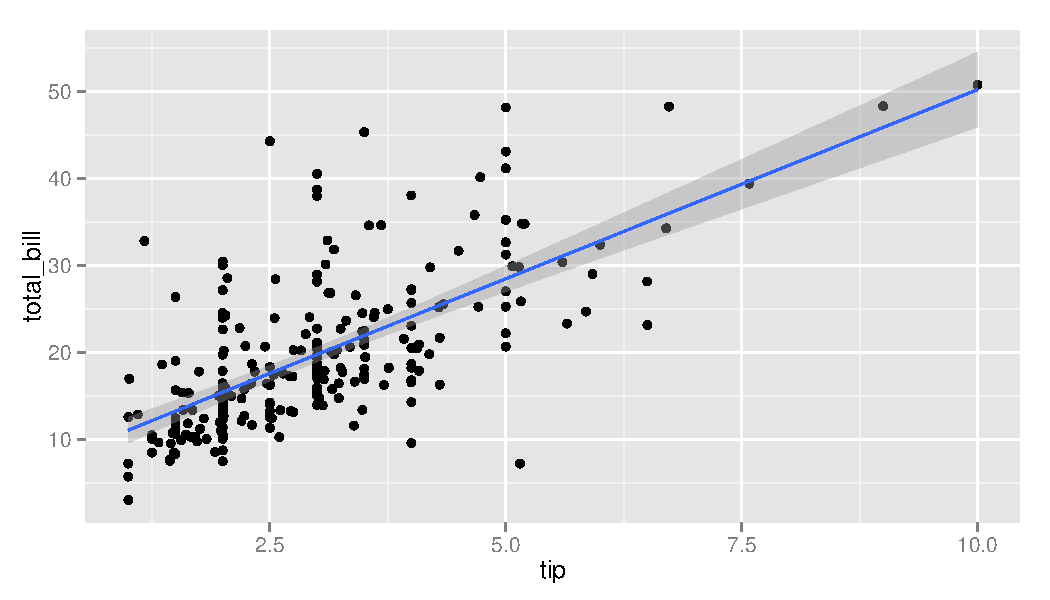
\includegraphics[width=\textwidth]{figure/kMEtipsscatterlm} 

\end{knitrout}

    \normalsize
\end{frame}

%-----------------------------------------------------------------------------

\begin{frame}[fragile]
    \frametitle{Rate of Tipping}
    
Tipping generally done using a rule of thumb based on a percentage of the total bill. We will make a new variable in the data set for the tipping rate = tip / total bill

\small
\begin{knitrout}\footnotesize
\definecolor{shadecolor}{rgb}{1, 1, 1}\color{fgcolor}\begin{kframe}
\begin{alltt}
\hlstd{tips}\hlopt{$}\hlstd{rate} \hlkwb{<-} \hlstd{tips}\hlopt{$}\hlstd{tip}\hlopt{/}\hlstd{tips}\hlopt{$}\hlstd{total_bill}
\hlcom{# What are the properties of this new variable for tipping rate?}
\hlkwd{summary}\hlstd{(tips}\hlopt{$}\hlstd{rate)}
\end{alltt}
\begin{verbatim}
##    Min. 1st Qu.  Median    Mean 3rd Qu.    Max. 
##  0.0356  0.1290  0.1550  0.1610  0.1910  0.7100
\end{verbatim}
\end{kframe}
\end{knitrout}

    \normalsize
\end{frame}

%-----------------------------------------------------------------------------

\begin{frame}[fragile]
    \frametitle{Tipping Rate Histogram}

Lets look distribution of tipping rate values with a histogram

\small
\begin{knitrout}\footnotesize
\definecolor{shadecolor}{rgb}{1, 1, 1}\color{fgcolor}\begin{kframe}
\begin{alltt}
\hlkwd{qplot}\hlstd{(rate,} \hlkwc{data} \hlstd{= tips,} \hlkwc{binwidth} \hlstd{=} \hlnum{0.05}\hlstd{)}
\end{alltt}
\end{kframe}
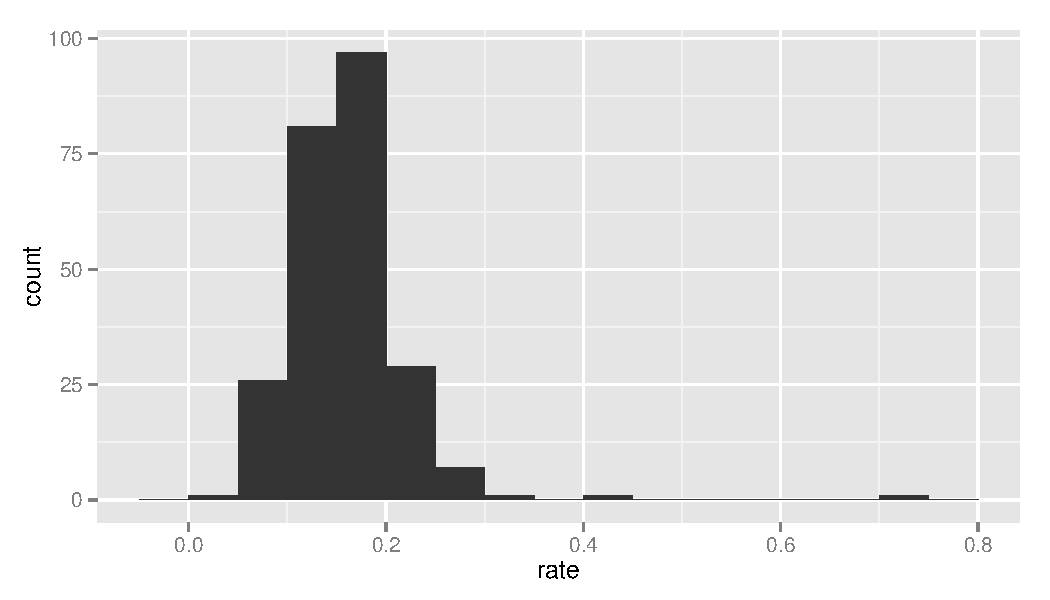
\includegraphics[width=\textwidth]{figure/kMEtipsratehisto} 

\end{knitrout}

    \normalsize
\end{frame}

%-----------------------------------------------------------------------------

\begin{frame}[fragile]
    \frametitle{Rate of Tipping}

One person tipped over 70\%, who are they?

\small
\begin{knitrout}\footnotesize
\definecolor{shadecolor}{rgb}{1, 1, 1}\color{fgcolor}\begin{kframe}
\begin{alltt}
\hlstd{tips[}\hlkwd{which.max}\hlstd{(tips}\hlopt{$}\hlstd{rate), ]}
\end{alltt}
\begin{verbatim}
##     total_bill  tip  sex smoker day   time size   rate
## 173       7.25 5.15 Male    Yes Sun Dinner    2 0.7103
\end{verbatim}
\end{kframe}
\end{knitrout}

    \normalsize
\end{frame}

%-----------------------------------------------------------------------------

\begin{frame}[fragile]
    \frametitle{Rates by Gender}

Look at the average tipping rate for men and women seperately

\small
\begin{knitrout}\footnotesize
\definecolor{shadecolor}{rgb}{1, 1, 1}\color{fgcolor}\begin{kframe}
\begin{alltt}
\hlkwd{mean}\hlstd{(tips}\hlopt{$}\hlstd{rate[tips}\hlopt{$}\hlstd{sex} \hlopt{==} \hlstr{"Male"}\hlstd{])}
\end{alltt}
\begin{verbatim}
## [1] 0.1577
\end{verbatim}
\begin{alltt}
\hlkwd{mean}\hlstd{(tips}\hlopt{$}\hlstd{rate[tips}\hlopt{$}\hlstd{sex} \hlopt{==} \hlstr{"Female"}\hlstd{])}
\end{alltt}
\begin{verbatim}
## [1] 0.1665
\end{verbatim}
\end{kframe}
\end{knitrout}

    \normalsize
\end{frame}

%-----------------------------------------------------------------------------

\begin{frame}[fragile]
    \frametitle{t-test}

There is a difference but is it statistically significant?

\small
\begin{knitrout}\footnotesize
\definecolor{shadecolor}{rgb}{1, 1, 1}\color{fgcolor}\begin{kframe}
\begin{alltt}
\hlkwd{t.test}\hlstd{(rate} \hlopt{~} \hlstd{sex,} \hlkwc{data} \hlstd{= tips)}
\end{alltt}
\begin{verbatim}
## 
## 	Welch Two Sample t-test
## 
## data:  rate by sex
## t = 1.143, df = 206.8, p-value = 0.2542
## alternative hypothesis: true difference in means is not equal to 0
## 95 percent confidence interval:
##  -0.006404  0.024084
## sample estimates:
## mean in group Female   mean in group Male 
##               0.1665               0.1577
\end{verbatim}
\end{kframe}
\end{knitrout}

    \normalsize
\end{frame}

%-----------------------------------------------------------------------------

\begin{frame}[fragile]
    \frametitle{Boxplots}

Perhaps we are interested if smokers tip at a different rate than non-smokers.  We could compare the rate values of each group with a side by side boxplot!

\small
\begin{knitrout}\footnotesize
\definecolor{shadecolor}{rgb}{1, 1, 1}\color{fgcolor}\begin{kframe}
\begin{alltt}
\hlkwd{qplot}\hlstd{(smoker, rate,} \hlkwc{geom} \hlstd{=} \hlstr{"boxplot"}\hlstd{,} \hlkwc{data} \hlstd{= tips)}
\end{alltt}
\end{kframe}
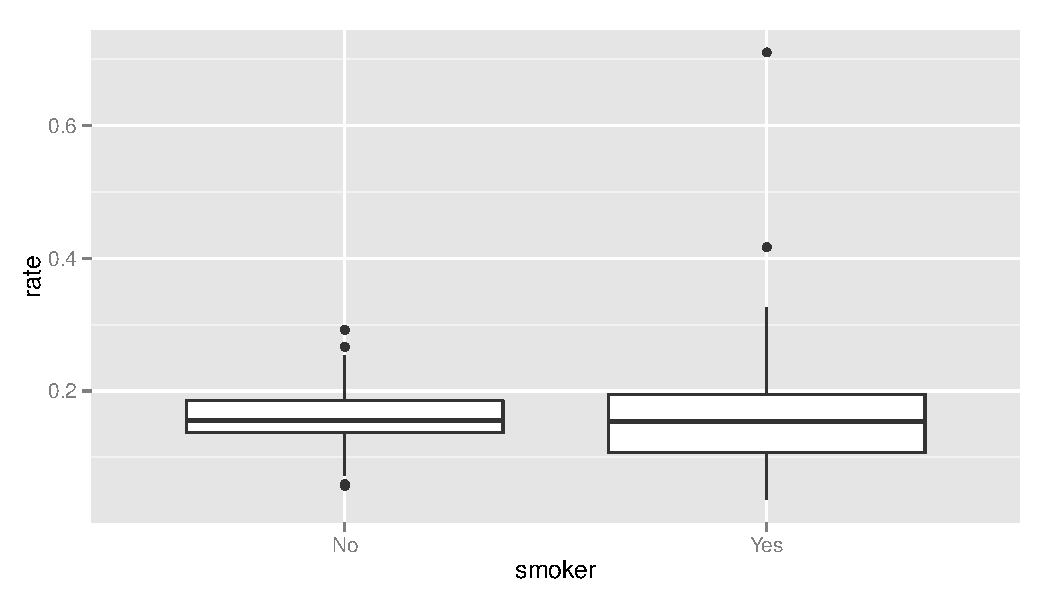
\includegraphics[width=\textwidth]{figure/kMEtipsboxplots} 

\end{knitrout}

    \normalsize
\end{frame}

%-----------------------------------------------------------------------------

\begin{frame}
    \frametitle{Your Turn}
    Try playing with chunks of code from RWorkshop1Tips.R to further investigate the tips data
    \begin{itemize}
        \item Get a summary of the total bill values
        \item Make side by side boxplots of tip rates for different days of the week
        \item Find the average tip value for smokers
    \end{itemize}    
\end{frame}




\end{document}
